\tikzset{every picture/.style={line width=0.75pt}} %set default line width to 0.75pt        

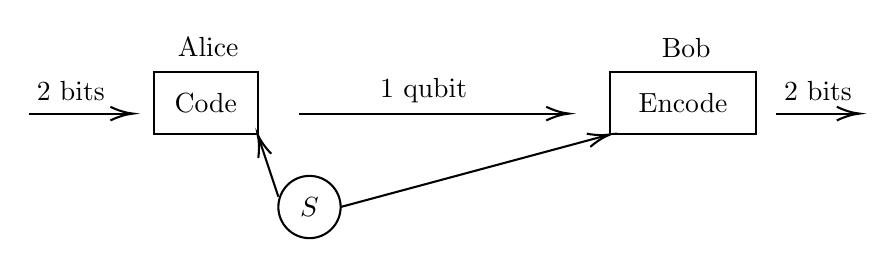
\begin{tikzpicture}[x=0.75pt,y=0.75pt,yscale=-1,xscale=1]
%uncomment if require: \path (0,300); %set diagram left start at 0, and has height of 300

%Shape: Rectangle [id:dp31062974555219114] 
\draw   (160,80) -- (210,80) -- (210,110) -- (160,110) -- cycle ;
%Shape: Rectangle [id:dp20682163383027818] 
\draw   (380,80) -- (450,80) -- (450,110) -- (380,110) -- cycle ;
%Shape: Circle [id:dp4743769670991709] 
\draw   (220,145) .. controls (220,136.72) and (226.72,130) .. (235,130) .. controls (243.28,130) and (250,136.72) .. (250,145) .. controls (250,153.28) and (243.28,160) .. (235,160) .. controls (226.72,160) and (220,153.28) .. (220,145) -- cycle ;
%Straight Lines [id:da5477596148170991] 
\draw    (220,140) -- (210.63,111.9) ;
\draw [shift={(210,110)}, rotate = 431.57] [color={rgb, 255:red, 0; green, 0; blue, 0 }  ][line width=0.75]    (10.93,-3.29) .. controls (6.95,-1.4) and (3.31,-0.3) .. (0,0) .. controls (3.31,0.3) and (6.95,1.4) .. (10.93,3.29)   ;

%Straight Lines [id:da9241704248293399] 
\draw    (250,145) -- (378.07,110.52) ;
\draw [shift={(380,110)}, rotate = 524.9300000000001] [color={rgb, 255:red, 0; green, 0; blue, 0 }  ][line width=0.75]    (10.93,-3.29) .. controls (6.95,-1.4) and (3.31,-0.3) .. (0,0) .. controls (3.31,0.3) and (6.95,1.4) .. (10.93,3.29)   ;

%Straight Lines [id:da19977175053033802] 
\draw    (100,100) -- (148,100) ;
\draw [shift={(150,100)}, rotate = 180] [color={rgb, 255:red, 0; green, 0; blue, 0 }  ][line width=0.75]    (10.93,-3.29) .. controls (6.95,-1.4) and (3.31,-0.3) .. (0,0) .. controls (3.31,0.3) and (6.95,1.4) .. (10.93,3.29)   ;

%Straight Lines [id:da30234793694339834] 
\draw    (230,100) -- (358,100) ;
\draw [shift={(360,100)}, rotate = 180] [color={rgb, 255:red, 0; green, 0; blue, 0 }  ][line width=0.75]    (10.93,-3.29) .. controls (6.95,-1.4) and (3.31,-0.3) .. (0,0) .. controls (3.31,0.3) and (6.95,1.4) .. (10.93,3.29)   ;

%Straight Lines [id:da08941647542512188] 
\draw    (460,100) -- (498,100) ;
\draw [shift={(500,100)}, rotate = 180] [color={rgb, 255:red, 0; green, 0; blue, 0 }  ][line width=0.75]    (10.93,-3.29) .. controls (6.95,-1.4) and (3.31,-0.3) .. (0,0) .. controls (3.31,0.3) and (6.95,1.4) .. (10.93,3.29)   ;


% Text Node
\draw (185,95) node  [align=left] {Code};
% Text Node
\draw (415,95) node  [align=left] {Encode};
% Text Node
\draw (235,145) node   {$S$};
% Text Node
\draw (120,89) node  [align=left] {2 bits};
% Text Node
\draw (290,89) node  [align=left] {1 qubit};
% Text Node
\draw (480,89) node  [align=left] {2 bits};
% Text Node
\draw (186.17,67.67) node  [align=left] {Alice};
% Text Node
\draw (416.5,68.33) node  [align=left] {Bob};

\end{tikzpicture}